\documentclass[beamer]{standalone}
\usepackage{circuitikz}
\begin{document}

\title[Electronics 1]{Filters}
\titlegraphic{
\includegraphics[height=0.5\textheight]{pics/brita}}

\begin{frame} 
  \titlepage
\end{frame}

\section{Fourier transform}
\begin{frame}
 \frametitle{Fourier series}
 \begin{block}{Definition of Fourier series of a function}
  If function $f(t)$ is \alert{periodic with period $T$}, then $a_n$ and $b_n$ exist such that
  \[ f(t) = \frac{a_0}{2} + \sum_{n=1,2,3,\ldots}^{+\infty} \left[ a_n \cos\left(\frac{2n\pi t}{T}\right) + b_n \sin\left(\frac{2n\pi t}{T}\right) \right] \]
  with
  \[ a_n = \frac{2}{T} \int_{-T/2}^{+T/2} f(t) \cos\left(\frac{2n\pi t}{T}\right) dt \]
  \[ b_n = \frac{2}{T} \int_{-T/2}^{+T/2} f(t) \sin\left(\frac{2n\pi t}{T}\right) dt \]
  The coefficients $a_n$ and $b_n$ indicate the strength of the harmonics with \alert{angular frequency $\omega_n = \frac{2n\pi}{T}$} or \alert{frequency $f_n = \frac{1}{T}$}.
 \end{block}
\end{frame}

\begin{frame}[t]
 \frametitle{Fourier series}
 \begin{block}{Example: Square wave}
  \begin{center}
   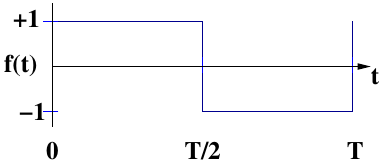
\includegraphics[width=0.5\textwidth]{pics/square_wave}
  \end{center}
  \[ f(t) = \frac{4}{\pi} \sum_{n=1,3,5,\ldots}^{+\infty} \frac{1}{n} \sin\left(\frac{2n\pi t}{T}\right) \]
 \end{block}
 \begin{block}{Live demo}
  \href{http://demonstrations.wolfram.com/FourierSeriesOfSimpleFunctions}{Fourier series of simple functions}
 \end{block}
\end{frame}

\begin{frame}[t]
 \frametitle{Fourier series}
 \begin{block}{Example: Square wave}
  \begin{center}
   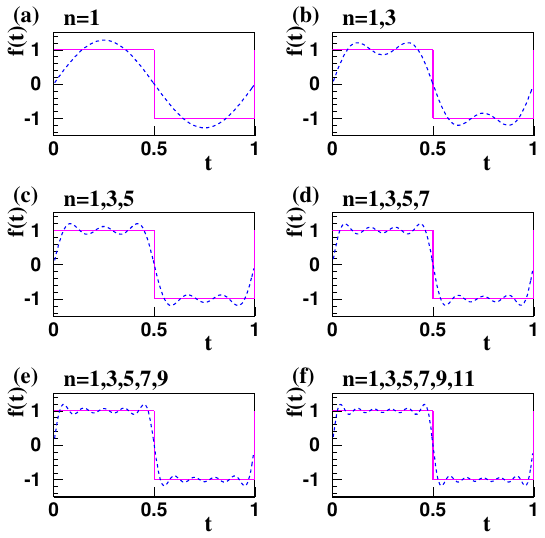
\includegraphics[width=0.48\textwidth]{pics/square_wave_approximation}
  \end{center}
  Filters (high-pass or low-pass) will have the effect of removing certain frequency harmonics.
 \end{block}
\end{frame}

\begin{frame}[t]
 \frametitle{Fourier series}
 \begin{block}{Power spectrum}
  Plot of coefficients $a_n$ and $b_n$ versus harmonic frequencies $\omega_n$
\only<1>{
 \[ f(t) = \frac{4}{\pi} \sum_{n=1,3,5,\ldots}^{+\infty} \frac{1}{n} \sin\left(\frac{2n\pi t}{T}\right) \quad \hbox{with}~b_n = \frac{4}{\pi}\frac{1}{n}, n=1,3,5,\ldots  \]
 }
 \end{block}
 \begin{block}<2>{Example: Square wave and triangle wave}
  \begin{center}
   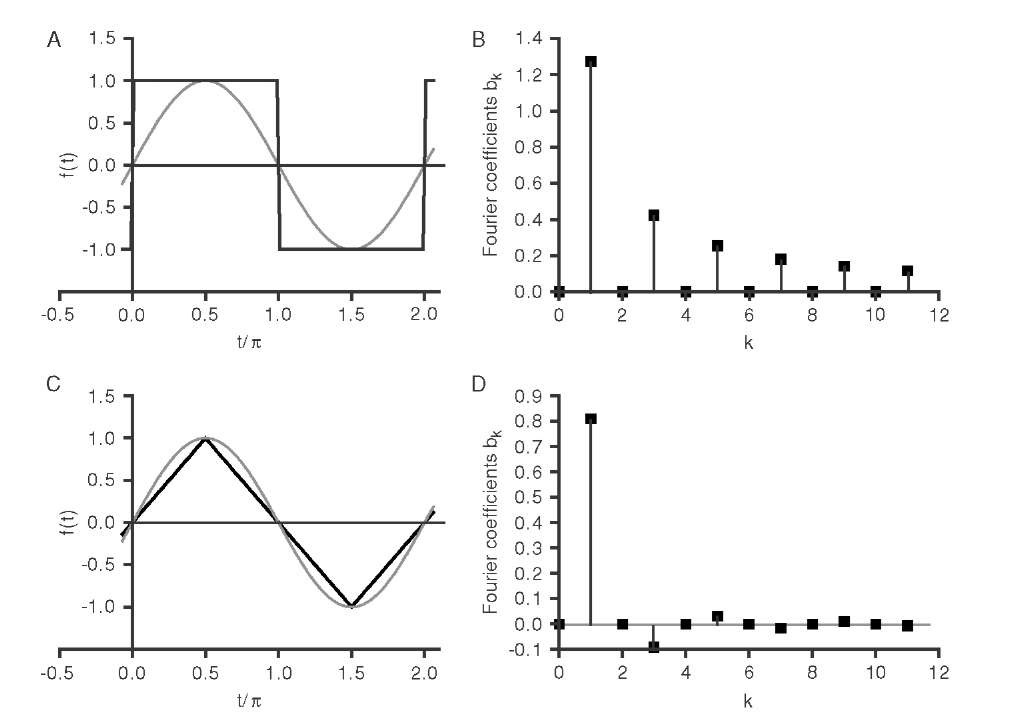
\includegraphics[width=0.65\textwidth]{pics/square_wave_b_n}
  \end{center}
 \end{block}
\end{frame}

\begin{frame}
 \frametitle{Fourier transform}
 \begin{block}{Definition of Fourier transform of a function}
  If function $f(t)$ goes to \alert{zero at $\pm \infty$}, then $F(\omega)$ exists such that
  \[ f(t) = \int^{+\infty}_{-\infty} F(\omega) e^{j \omega t} d\omega \]
  with
  \[ F(\omega) = \int^{+\infty}_{-\infty} f(t) e^{-j \omega t} dt \]
 \end{block}
 \begin{block}{Power spectrum}
  The Fourier transform $F(\omega)$ gives the strength \alert{for all frequencies}, not just the harmonics of some fundamental frequency.
 \end{block}
 \begin{block}{Live demo}
  \href{http://demonstrations.wolfram.com/ComparingFourierSeriesAndFourierTransform/}{Comparing Fourier series and Fourier transform}
 \end{block}
\end{frame}

\begin{frame}
 \frametitle{Fourier transform}
 \begin{block}{Example: Sine/cosine wave with $\omega_0$}
  Fourier transform is single ``$\delta$-spike'' at $\omega = \omega_0$, because no other frequency components are present.
  \[ f(t) = \cos\omega_0 t \Rightarrow F(\omega) = 0 \quad \hbox{for} \quad \omega \ne \omega_0 \]
 \end{block}
 \begin{block}{Example: Single square pulse (and basically every signal)}
  Because all frequency components are represented in the discontinuous step, the Fourier transform is non-zero for all value of $\omega$.
 \end{block}
 \begin{block}{Distortion due to systems}
  When a single pulse passes through a system that affects some frequency ranges differently, it will be distorted.
 \end{block}
\end{frame}

\begin{frame}
\frametitle{Fourier transform}
\begin{center}
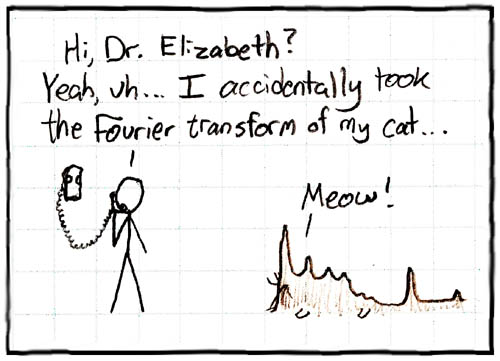
\includegraphics[height=0.7\textheight]{pics/fourier} \\
\href{http://xkcd.com/26}{xkcd/26}
\end{center}
\end{frame}


\section{Transfer function and Bode plots}
\begin{frame}
 \frametitle{Transfer function}
   \begin{columns}[t]
    \begin{column}{.45\textwidth}
     Time domain
     \begin{figure}
      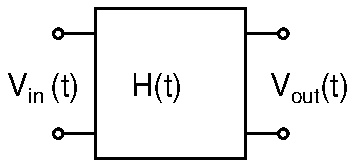
\includegraphics[width=0.55\textwidth]{./circuits/black_box_transfer_in_time.pdf}
     \end{figure}
     \[V_{out}(t)=\int^t_{-\infty} H(t-\tau) V_{in}(\tau) d \tau \]
    \end{column}
    \begin{column}{.45\textwidth}
     Frequency domain
     \begin{figure}
      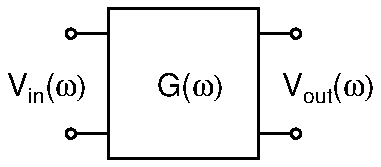
\includegraphics[width=0.55\textwidth]{./circuits/black_box_transfer_in_freq.pdf}
     \end{figure}
     \[V_{out}(\omega)=G(\omega) V_{in}(\omega) \]
     Where $G$ is complex transfer function or gain.
    \end{column}
   \end{columns}
   \begin{block}{Definition of gain}
    \[ G(\omega)=\frac{V_{out}(\omega)}{V_{in}(\omega)} = |G(\omega)| e^{j \phi(\omega)} \]
   \end{block}
   Often used values of $G$ in dB, with
   \[ dB = 20 \log_{10} (|G(w)|) \]
\end{frame}

\section{Filters}

 
\begin{frame}
 \frametitle{Simple example: RC low-pass filter}
     \begin{figure}
      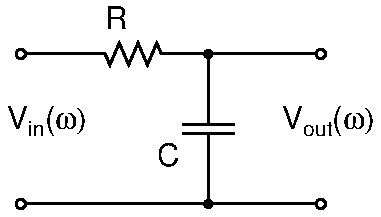
\includegraphics[width=0.25\textwidth]{./circuits/rc_low_pass.pdf}
     \end{figure}
    \[ G(\omega)
    =\frac{V_{out}(\omega)}{V_{in}(\omega)}
    = \frac{\frac{1}{j \omega C}}{R+\frac{1}{j \omega C}} 
    = \frac{1}{j \omega R C} \frac{1}{1+\frac{1}{j \omega R C}}
    = \frac{1}{1+j \omega R C}
    \]
    Define $\omega_{3dB}=\frac{1}{RC}$
    \[ G(\omega)
    = \frac{1}{1+j\frac{\omega}{\omega_{3dB}}}
    = \frac{1}{\sqrt{1+\frac{\omega^2}{\omega_{3dB}^2}}} e^{j \phi} ,
    \phi = atan (-\frac{\omega}{\omega_{3dB}})
    \]
    What does $\omega_{3dB}$ represent?
    \[
    |G(\omega=\omega_{3dB})|=20 \log_{10}\left(\frac{1}{\sqrt{1+1}}\right)
    =20 \log_{10}\left(\frac{1}{\sqrt{2}}\right)=-3 dB
    \]
\end{frame}


\begin{frame}
\frametitle{RC low-pass filter at $\omega=0.1/RC$}
\begin{columns}[c]
 \begin{column}{.55\textwidth}
  Signal vs time
  \begin{figure}
   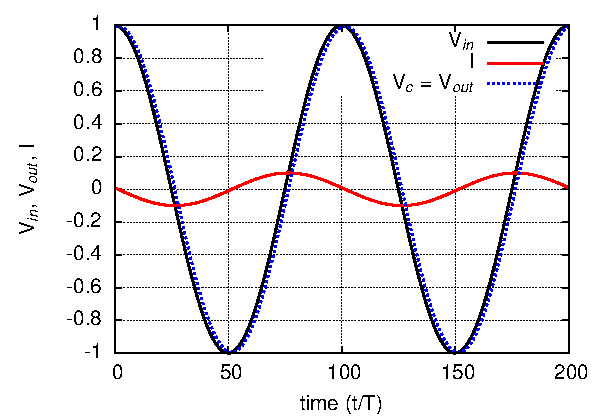
\includegraphics[angle=0,width=0.90\textwidth]{./plots/i_v_vr_w=_1rc}
  \end{figure}
 \end{column}
 \begin{column}{.45\textwidth}
  Lissajous plot
  \begin{figure}
   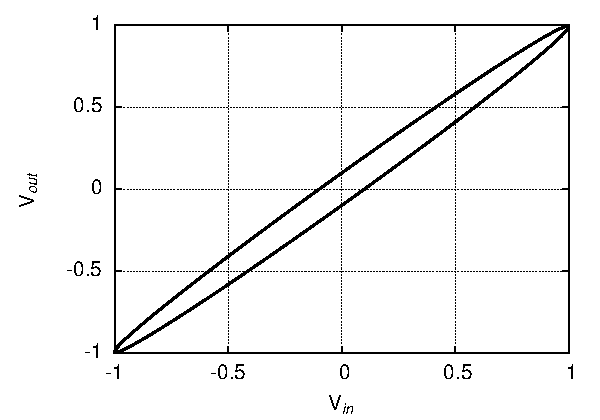
\includegraphics[angle=0,width=0.90\textwidth]{./plots/vc_vs_vin_w=_1rc}
  \end{figure}
 \end{column}
\end{columns}
\end{frame}

\begin{frame}
\frametitle{RC low-pass filter at $\omega=1/RC$}
\begin{columns}[c]
 \begin{column}{.55\textwidth}
  Signal vs time
  \begin{figure}
   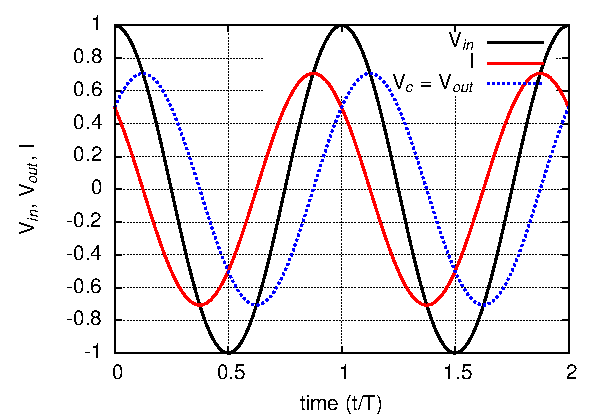
\includegraphics[angle=0,width=0.90\textwidth]{./plots/i_v_vr_w=rc}
  \end{figure}
 \end{column}
 \begin{column}{.45\textwidth}
  Lissajous plot
  \begin{figure}
   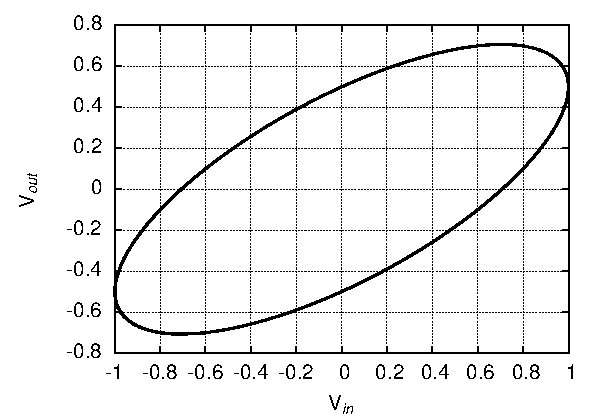
\includegraphics[angle=0,width=0.90\textwidth]{./plots/vc_vs_vin_w=rc}
  \end{figure}
 \end{column}
\end{columns}
\end{frame}

\begin{frame}
\frametitle{RC low-pass filter at $\omega=10/RC$}
\begin{columns}[c]
 \begin{column}{.55\textwidth}
  Signal vs time
  \begin{figure}
   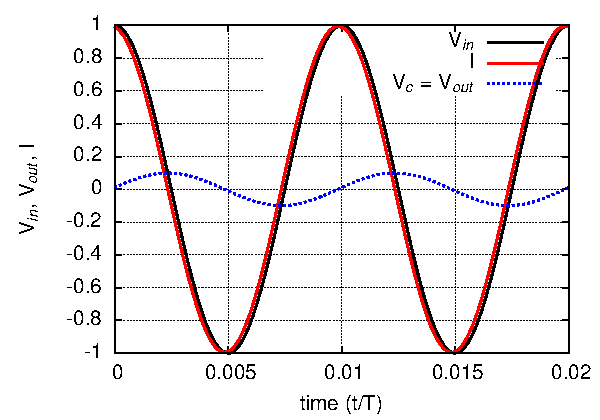
\includegraphics[angle=0,width=0.90\textwidth]{./plots/i_v_vr_w=10rc}
  \end{figure}
 \end{column}
 \begin{column}{.45\textwidth}
  Lissajous plot
  \begin{figure}
   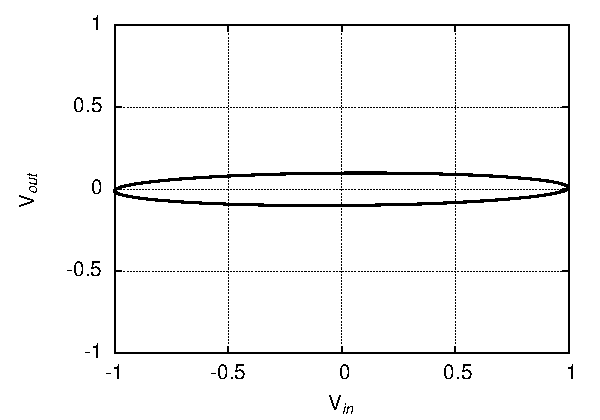
\includegraphics[angle=0,width=0.90\textwidth]{./plots/vc_vs_vin_w=10rc}
  \end{figure}
 \end{column}
\end{columns}
\end{frame}

\begin{frame}
\frametitle{Bode plots}
 \begin{block}{What are Bode plots?}
  Plots of magnitude and phase of the transfer function, where
  $|G|$ is often plotted in dB
 \end{block}
   \begin{columns}[c]
    \begin{column}{.25\textwidth}
     \begin{figure}
      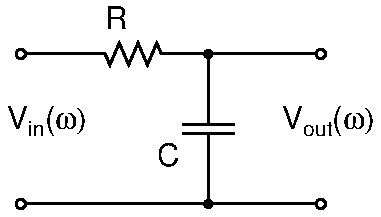
\includegraphics[width=1.00\textwidth]{./circuits/rc_low_pass.pdf}
     \end{figure}
    \[ G(\omega)
    = \frac{1}{1+j\frac{\omega}{\omega_{3dB}}}
    \]
    \end{column}
    \begin{column}{.75\textwidth}
      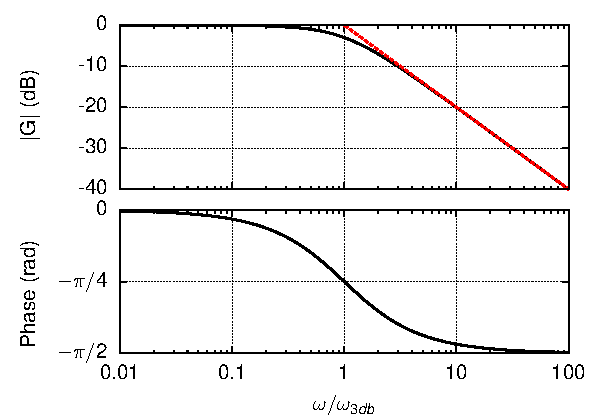
\includegraphics[angle=0,width=1.00\textwidth]{./plots/rc_low_pass_bode.pdf}
    \end{column}
   \end{columns}
\end{frame}

\begin{frame}
 \frametitle{Bode plots: Why in dB?}
 \begin{block}{Problem}
  You want to measure the 1\,$\mu$V fluctuations caused by the fast motion of atoms in an optical trap (at 6\,kHz).  The entire system is powered by 110\,V, 60\,Hz power from the grid, and you will need to filter this out.  What factor of 60\,Hz suppression noise do you need (in dB)?
 \end{block}
 \begin{block}<2>{Discussion}
  \begin{itemize}
   \item Let's assume that you want a 10-to-1 signal-to-noise ratio, then the maximum voltage at 60\,Hz is 100\,nV.  You need a suppression by a factor $10^9$, or 180\,dB.
   \item You look in your lab and find some RC filters with a factor 177.8 suppression.  How many would you need?
   \item You look a bit further and find some RC filters with 45\,dB suppression.  How many of these would you need?
   \item Will it work?  (We'll come back to this\ldots)
  \end{itemize}
 \end{block}
\end{frame}
 
\begin{frame}[t]
 \frametitle{Bode plots: Filter theory (a little bit)}
 \begin{block}{Characteristics of a Bode plot}
  \begin{itemize}
   \item Straight lines in log-log plots (major advantage of dB scale)
   \item 3dB frequencies are cut-off points: $\omega_{3dB}$ where $|G(\omega)| = 3\,dB$
   \item Power roll-off: goes like $\omega^n$ ($n$ is the order of the filter)
   \begin{itemize}
    \item For first-order filters, $n = 1$, and one decade in $\omega$ corresponds to a 20\,dB reduction
   \end{itemize}
  \end{itemize}
 \end{block}
 \begin{block}{Filter theory in a nut shell}
  The gain $G(\omega)$ can be written as $G(\omega) = A \prod_n \frac{(\omega + j z_n)^{a_n}}{(\omega + j p_n)^{b_n}}$ with zeroes $z_n$ and poles $p_n$ (with multiplicities $a_n$ and $b_n$).
  \begin{itemize}
   \item Start with constant magnitude for $\omega = 0$
   \item Each pole or zero will result in a 20\,dB/decade change of slope per multiplicity (down for poles, up for zeroes).
   \item At each pole or zero you adjust the plot by 3\,dB.
  \end{itemize}
 \end{block}
\end{frame}


\begin{frame}
\frametitle{RC high-pass filter}
   \begin{columns}[c]
    \begin{column}{.25\textwidth}
     \begin{figure}
      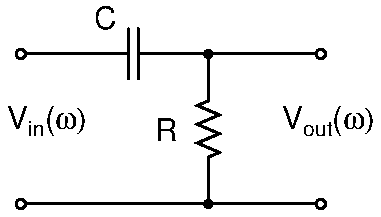
\includegraphics[width=1.00\textwidth]{./circuits/rc_high_pass.pdf}
     \end{figure}
    \end{column}
    \begin{column}{.75\textwidth}
      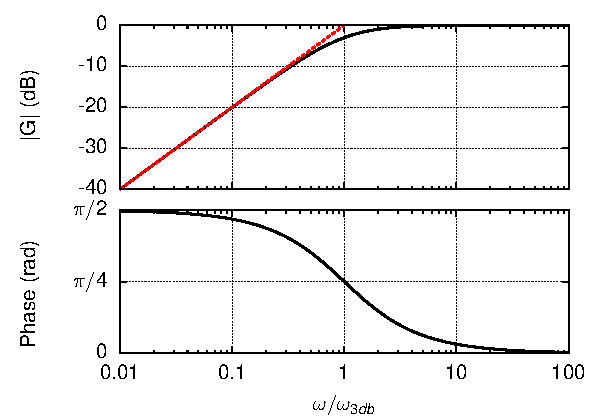
\includegraphics[angle=0,width=1.00\textwidth]{./plots/rc_high_pass_bode.pdf}
    \end{column}
   \end{columns}
    \[ G(\omega)
    =\frac{V_{out}(\omega)}{V_{in}(\omega)}
    = \frac{R}{R+\frac{1}{j \omega C}} 
    = \frac{j \omega R C}{1+j \omega R C}
    = \frac{j \frac{\omega}{\omega_{3dB}}}{1+j\frac{\omega}{\omega_{3dB}}}
    \]
    with $\omega_{3dB}=\frac{1}{RC}$
\end{frame}

\begin{frame}
 \frametitle{Bode plots: Filter theory (a little bit)}
 \begin{block}{Drawing the RC high-pass filter Bode diagram}
  \begin{itemize}
   \item Zero at $\omega = 0$ (multiplicity of 1).
   \item Line from $\omega = 0$ to $\omega = \omega_{3dB}$ increases by 20\,dB/decade.
   \item Pole at $\omega = \omega_{3dB}$ (multiplicity of 1).
   \item Slope changes by 20\,dB/decade, then remains constant for $\omega \to \infty$.
  \end{itemize}
 \end{block}
\end{frame}


\begin{frame}
\frametitle{RL filters}
   \begin{columns}[c]
    \begin{column}{.50\textwidth}
     RL low-pass filter
     \begin{figure}
      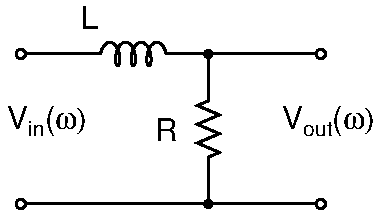
\includegraphics[width=0.50\textwidth]{./circuits/rl_low_pass.pdf}
     \end{figure}
     \[
     G(\omega) 
     = \frac{R}{R+j\omega L},
     \omega_{3dB}=\frac{R}{L}
     \]
     \vskip -.3in
     \begin{figure}
      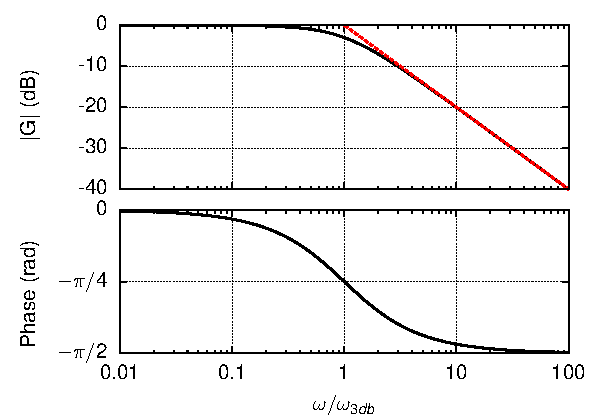
\includegraphics[angle=0,width=1.0\textwidth]{./plots/rl_low_pass_bode.pdf}
     \end{figure}
    \end{column}
    \begin{column}{.50\textwidth}
     RL high-pass filter
     \begin{figure}
      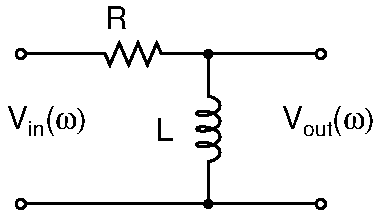
\includegraphics[width=0.5\textwidth]{./circuits/rl_high_pass.pdf}
     \end{figure}
     \[
     G(\omega)
     = \frac{j \omega L}{R+j\omega L}
     \]
     \vskip -.3in
     \begin{figure}
      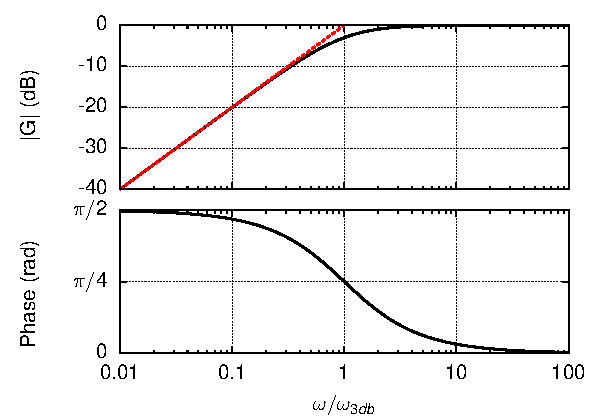
\includegraphics[angle=0,width=1.0\textwidth]{./plots/rl_high_pass_bode.pdf}
     \end{figure}
    \end{column}
   \end{columns}
\end{frame}

\subsection{Loaded vs unloaded filter}
\begin{frame}
 \frametitle{Voltage divider}
 \begin{columns}[c]
  \begin{column}{.4\textwidth}
   \includegraphics<1>[height=2in]{./pics/unloaded_voltage_divider}
   \includegraphics<2>[height=2in]{./pics/loaded_voltage_divider}
  \end{column}
  \begin{column}{.6\textwidth}
   \begin{itemize}
    \item Gain $G = \frac{V_{out}}{V_{in}} = \frac{R_2}{R_1 + R_2}$
    \item What is the resistance $V_{in}$ sees?
    \[ R_{in} = R_1 + R_2 \]
    \item What is the Th\'{e}venin resistance?
    \[ R_{out} = R_{1 \parallel 2} \]
    \item<2> Rule of 10: if $R_L > 10 R_{out}$, then the voltage $V_{out}$ will be virtually unchanged
   \end{itemize}
  \end{column}
 \end{columns}
\end{frame}

\begin{frame}
 \frametitle{Input and output impedances}
 \begin{center}
  \begin{circuitikz}
   \draw (-2,2) node[left]{$v_{in}$} to[R,l=$R$,o-] (0,2) to[C,l=$C$] (0,0.5) node[ground]{};
   \draw (0,2) to[short,-o] (1,2) node[right]{$v_{out}$};
  \end{circuitikz}
 \end{center}
 \begin{columns}[t]
  \begin{column}{0.48\textwidth}
   \begin{block}{Input impedance $Z_{in}$}
    \begin{itemize}
     \item What is the impedance a driving circuit sees?
     \item Assume large load $Z_L$ is connected (rule of 10).
     \item<2-> R and C in series: $Z_{in} = R + \frac{1}{j\omega C}$
    \end{itemize}
   \end{block}
  \end{column}
  \begin{column}{0.48\textwidth}
   \begin{block}{Output impedance $Z_{out}$}
    \begin{itemize}
     \item What is the Th\'evenin impedance of the filter?
     \item Assume small internal resistance of driving circuit.
     \item<3-> R and C in parallel: $Z_{out} = \frac{V_{Th}}{I_{N}} = \frac{R}{1 + j\omega RC}$
    \end{itemize}
   \end{block}
  \end{column}
 \end{columns}
\end{frame}

\begin{frame}
 \frametitle{Filters chain}
 \begin{figure}
  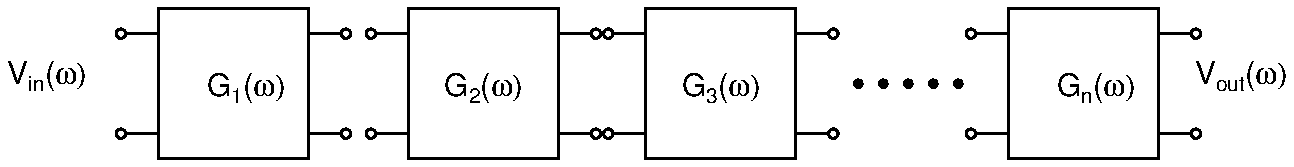
\includegraphics[angle=0,width=1.0\textwidth]{./circuits/black_box_transfer_in_freq_chain.pdf}
 \end{figure}
 Technically next stage loads the previous and it is quite hard to
 calculate total transfer function.

 However we use rule of 10 to avoid overloading the previous filter.\\
 Every next stage resistor $|Z_{in,i+1}| > 10 |Z_{out,i}|$ we can approximate
 \[
 G_t(\omega) \approx G_1(\omega) G_2(\omega) G_3(\omega) \cdots G_n(\omega)
 \]
\end{frame}

\frame
{ \frametitle{ Example band pass filter}
\begin{figure}
 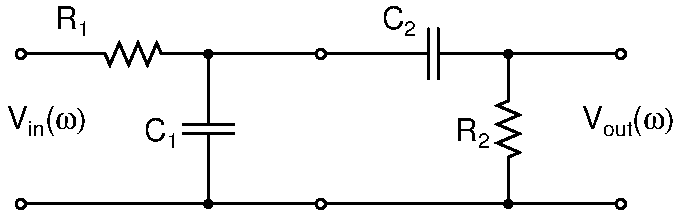
\includegraphics[angle=0,width=0.5\textwidth]{./circuits/band_pass_filter.pdf}
\end{figure}
\begin{columns}
 \begin{column}{.50\textwidth}
  \[
  G_t(\omega) \approx G_1(\omega) G_2(\omega) 
  \]
  \[
  G_t(\omega) \approx
  \frac{1}{1+j\frac{\omega}{\omega_{1_{3dB}}}}
  \frac{j \frac{\omega}{\omega_{2_{3dB}}}}{1+j\frac{\omega}{\omega_{2_{3dB}}}}
  \]
  For $R_1=1 k\Omega, R_2=100 k\Omega$,\\
  $C_1=C_2=.01 \mu F$
 \end{column}
 \begin{column}{.50\textwidth}
  \vskip -.2in
  \begin{figure}
   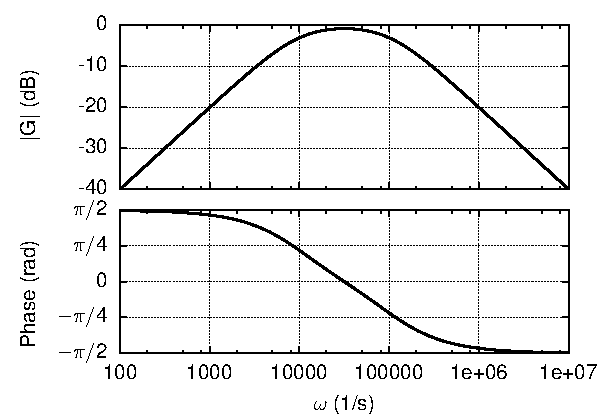
\includegraphics[angle=0,width=1.0\textwidth]{./plots/rc_band_pass_bode.pdf}
  \end{figure}
 \end{column}
\end{columns}
}

\frame
{ \frametitle{Notch filter - Band stop filter}
\vskip -0.4in
\begin{columns}
 \begin{column}{.250\textwidth}
  \begin{figure}
   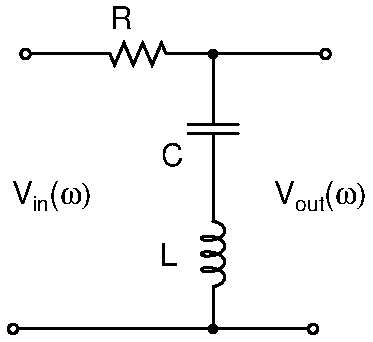
\includegraphics[angle=0,width=1.00\textwidth]{./circuits/rlcnotch.pdf}
  \end{figure}
  \[
  \omega_0=\frac{1}{\sqrt{LC}}
  \]
 \end{column}
 \begin{column}{.750\textwidth}
  \begin{figure}
   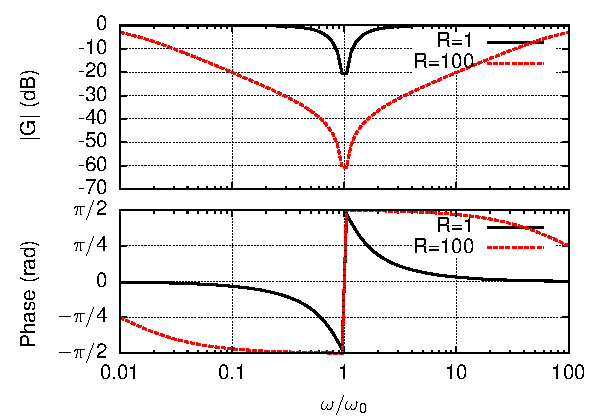
\includegraphics[angle=0,width=1.0\textwidth]{./plots/rlc_notch_bode.pdf}
  \end{figure}
 \end{column}
\end{columns}
\alert{It is impossible to make band stop filter with $G\approx1$ outside
of stop band with only simple combinations of low and high-pass filters.}
R, L, and C combo is required or a complicated network of R-C, R-L elements.
}

\subsection{RLC filters}
\begin{frame}
 \frametitle{RLC filters}
 \begin{columns}
  \begin{column}{0.4\textwidth}
   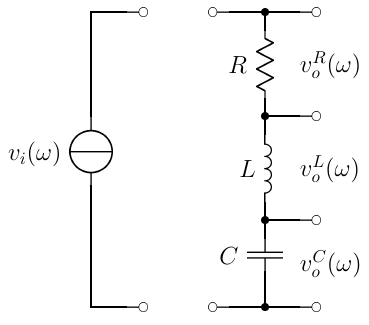
\includegraphics[width=\textwidth]{pics/RLC_circuit}
  \end{column}
  \begin{column}{0.6\textwidth}
   \begin{itemize}
    \item $\omega_{LC} = \frac{1}{\sqrt{LC}}$
    \item $\omega_{RC} = \frac{1}{RC}$
    \item $\omega_{RL} = \frac{R}{L}$
   \end{itemize}
   Note: $\omega_{RC} \omega_{RL} = \omega^2_{LC}$
  \end{column}
 \end{columns}
 \begin{block}{Three output voltages}
  \begin{columns}
   \begin{column}{0.5\textwidth}
    \begin{itemize}
     \item $v_o^R(\omega)$ across resistor
     \item $v_o^L(\omega)$ across inductor
     \item $v_o^C(\omega)$ across capacitor
    \end{itemize}
   \end{column}
   \begin{column}{0.5\textwidth}
    Typically $R$ and $L$ in one component, so measure $v_o^R(\omega) + v_o^L(\omega)$
   \end{column}
  \end{columns}
 \end{block}
\end{frame}

\begin{frame}
 \frametitle{RLC filters}
 \begin{block}{Total impedance}
  \begin{equation*}
   Z_{tot} = R + j\omega L + \frac{1}{j\omega C} = R \left[ 1 - j\frac{\omega_{RC}}{\omega} \left( 1 - \frac{\omega^2}{\omega_{LC}^2} \right) \right]
  \end{equation*}
 \end{block}
 \begin{block}{Voltage divider: gain across capacitor}
  \begin{equation*}
   G_C(\omega) = \frac{Z_C}{Z_{tot}} = \frac{1}{j\omega RC\left[ 1 - j\frac{\omega_{RC}}{\omega} \left( 1 - \frac{\omega^2}{\omega_{LC}^2} \right) \right]} = \frac{1}{\left( 1 - \frac{\omega^2}{\omega_{LC}^2} \right) + j\frac{\omega}{\omega_{RC}}}
  \end{equation*}
  \begin{eqnarray*}
   |G_C(\omega)| & = & \frac{1}{\sqrt{ \left(1 - \omega^2/\omega_{LC}^2 \right)^2 + \omega^2/\omega^2_{RC}}} \\
   \phi_C & = & \tan^{-1} \frac{- \omega/\omega_{RC}}{1 - \omega^2/\omega_{LC}^2}
  \end{eqnarray*}
 \end{block}
\end{frame}

\begin{frame}
 \frametitle{RLC filters: gain across capacitor}
 \begin{block}{Resonance at $\omega = \omega_{LC}$}
  \begin{itemize}
   \item $|G_C(\omega)| = \frac{\omega_{RC}}{\omega_{RL}} = \sqrt{\frac{L}{R^2 C}}$ large for $R$ small
   \item $\phi_C = -\frac{\pi}{2}$
  \end{itemize}
 \end{block}
 \begin{block}{Low frequency limit}
  \begin{itemize}
   \item $|G_C(\omega)| \to 1$
   \item $\phi_C \to 0$
  \end{itemize}
 \end{block}
 \begin{block}{High frequency limit}
  \begin{itemize}
   \item $|G_C(\omega)| \to \frac{\omega^2_{LC}}{\omega^2}$
   \item $\phi_C \to -\pi$
  \end{itemize}
 \end{block}
\end{frame}

\begin{frame}
 \frametitle{RLC filters: gain across capacitor}
 \begin{center}
  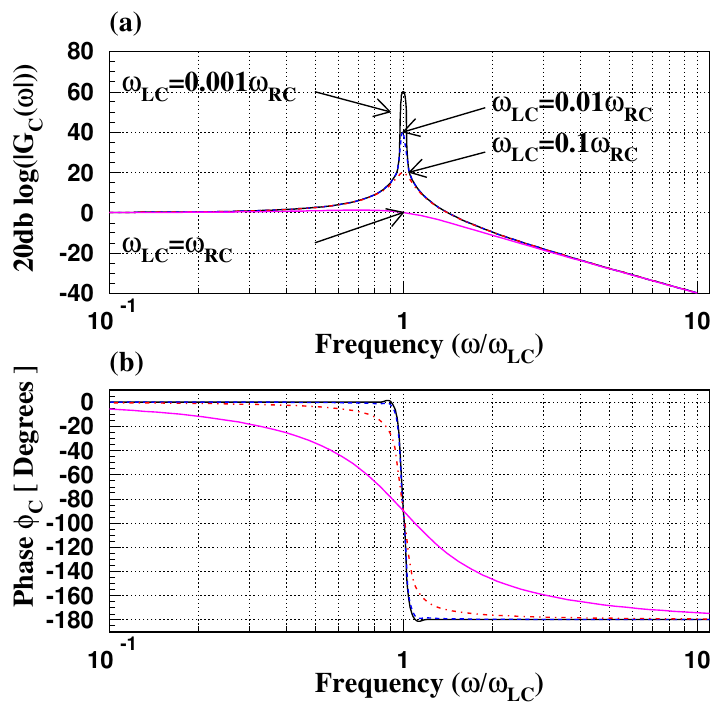
\includegraphics[width=0.6\textwidth]{pics/RLC_bode_capacitor}
 \end{center}
\end{frame}

\begin{frame}
 \frametitle{RLC filters}
 \begin{block}{Voltage divider: gain across inductor}
  \begin{equation*}
   G_L(\omega) = \frac{Z_L}{Z_{tot}} = \frac{j\omega L}{R\left[ 1 - j\frac{\omega_{RC}}{\omega} \left( 1 - \frac{\omega^2}{\omega_{LC}^2} \right) \right]} = \frac{1}{\left( 1 - \frac{\omega^2_{LC}}{\omega^2} \right) + j\frac{\omega_{RL}}{\omega}}
  \end{equation*}
  \begin{eqnarray*}
   |G_L(\omega)| & = & \frac{1}{\sqrt{ \left(1 - \omega_{LC}^2/\omega^2 \right)^2 + \omega_{RL}^2/\omega^2}} \\
   \phi_L & = & \tan^{-1} \frac{\omega_{RL}/\omega}{1 - \omega_{LC}^2/\omega^2}
  \end{eqnarray*}
 \end{block}
\end{frame}

\begin{frame}
 \frametitle{RLC filters: gain across inductor}
 \begin{block}{Resonance at $\omega = \omega_{LC}$}
  \begin{itemize}
   \item $|G_L(\omega)| = \frac{\omega_{LC}}{\omega_{RL}} = \sqrt{\frac{L}{R^2 C}}$ large for $R$ small
   \item $\phi_L = \frac{\pi}{2}$
  \end{itemize}
 \end{block}
 \begin{block}{Low frequency limit}
  \begin{itemize}
   \item $|G_L(\omega)| \to \frac{\omega^2}{\omega_{LC}^2}$
   \item $\phi_L \to \pi$
  \end{itemize}
 \end{block}
 \begin{block}{High frequency limit}
  \begin{itemize}
   \item $|G_L(\omega)| \to 1$
   \item $\phi_L \to 0$
  \end{itemize}
 \end{block}
\end{frame}

\begin{frame}
 \frametitle{RLC filters: gain across inductor}
 \begin{center}
  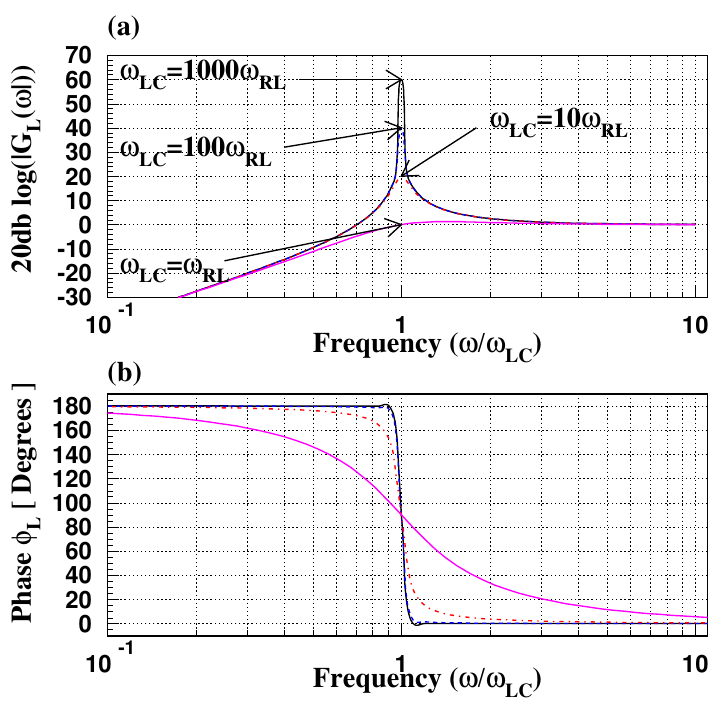
\includegraphics[width=0.6\textwidth]{pics/RLC_bode_inductor}
 \end{center}
\end{frame}

\begin{frame}
 \frametitle{RLC filters: gain larger than 0\,dB}
 \begin{columns}
  \begin{column}{0.5\textwidth}
   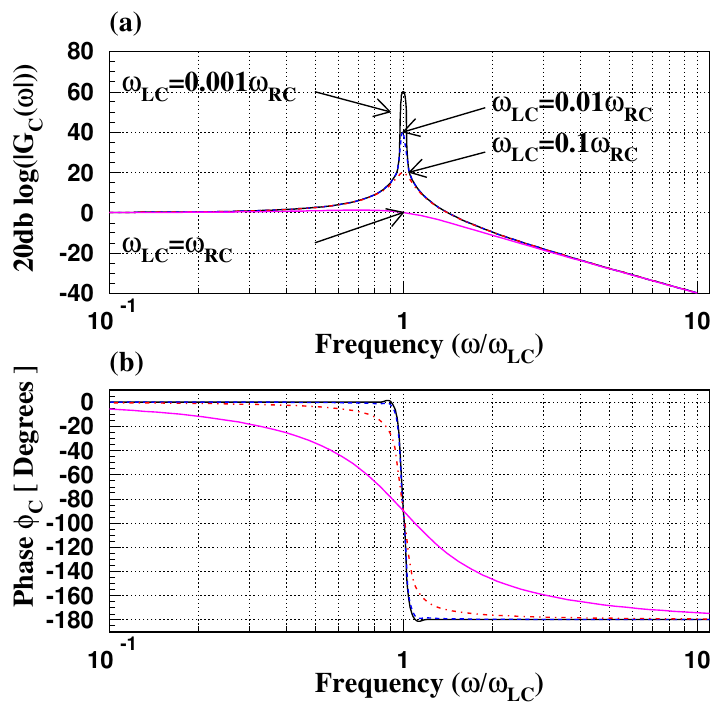
\includegraphics[width=\textwidth]{pics/RLC_bode_capacitor}   
  \end{column}
  \begin{column}{0.5\textwidth}
   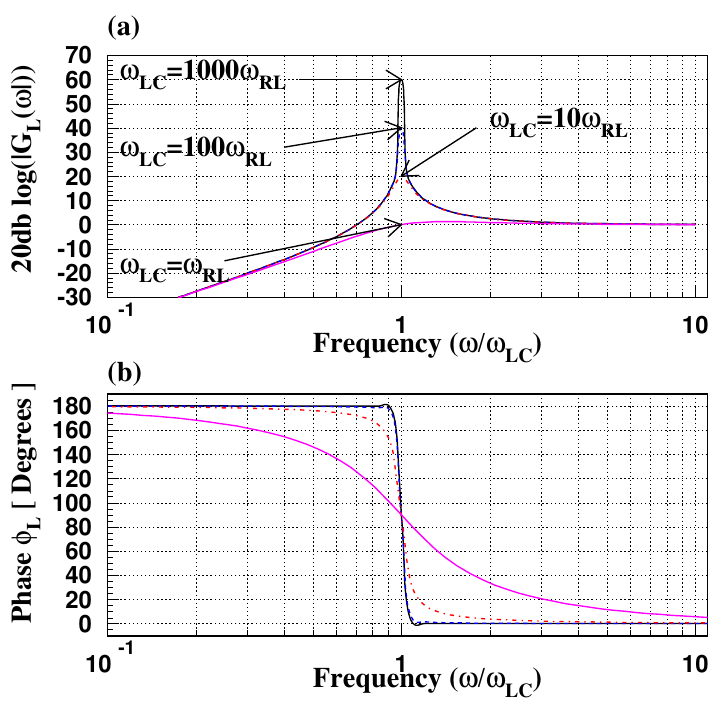
\includegraphics[width=\textwidth]{pics/RLC_bode_inductor}
  \end{column}
 \end{columns}
 \begin{block}{Gain larger than 1}
  Possible when the phase is opposite:
  \begin{itemize}
   \item $v_C(t) + v_L(t) = 0$
  \end{itemize}
 \end{block}
\end{frame}


\end{document}
